%!\subsection{Quantitative complexity Analysis}
%    \label{subsec:ComplexityImageAnalysis}
%    %!\subsection{Quantitative complexity Analysis}
%    \label{subsec:ComplexityImageAnalysis}
%    %!\subsection{Quantitative complexity Analysis}
%    \label{subsec:ComplexityImageAnalysis}
%    %!\subsection{Quantitative complexity Analysis}
%    \label{subsec:ComplexityImageAnalysis}
%    \input{Text/ComplexityImageAnalysis.tex}

We have previously stated the argument that the history of architecture, and the essence of architecture evolution, consists of an ever-changing interplay between simplicity and complexity.

we have explored the theoretical definition and revisioned the different approach towards facades and ornamentation from the perspective of some of the most prominant architectural style across history and the views of their most recognized representatives.

the conclusion from this literature analysis was that the current trend in architecture tilts towards a new revival of complexity however it might look like a suibjective view and insinuate perhaps some biased towards this outcome .

for this reason an additional quantitatvie analysis using Image complexity analysis was conducted using as input images of the most representative buildings across epochs and styles.

For this the complexity image analysis that assigns a complexity value governed by the complexity definition that Complexity of an image is governed by spatial, frequency and color information present in the image.

Scanpath based image complexity analysis determines human visual behavior that could lead to development of interactive and intelligent systems.\cite{Ishrat2020}

The objective of current research work is to establish the complexity of the given set of images while target objects are searched and to present analysis ofgaze search pattern.
To achieve these objectives a remote gaze estimation and analysis model has been proposed for scanpath identification and analysis.\cite{Ishrat2020}

%% Figure of Complexity graph
     \begin{figure*}[htb]
          \centering
          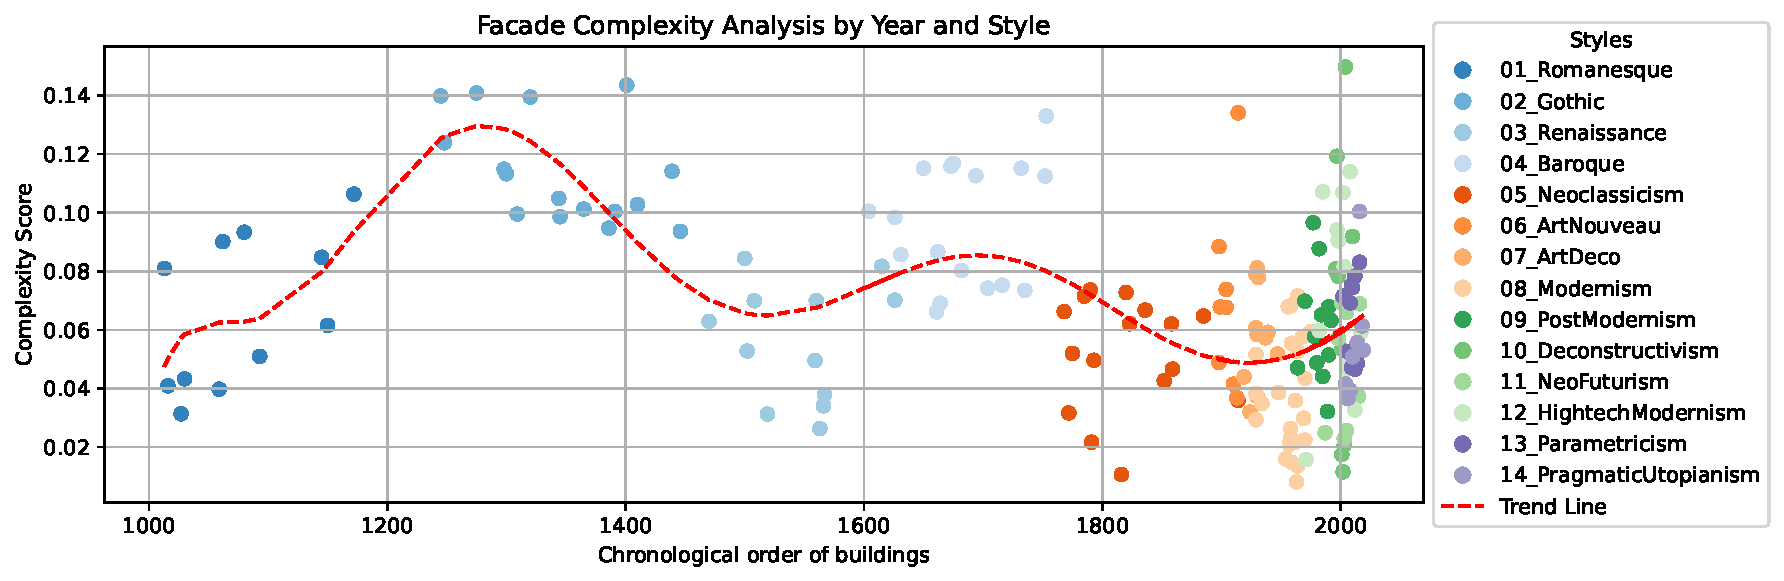
\includegraphics[width= \linewidth]{Graphs/complexitygraph}
          \caption{Contemporary architecture. An era of exploration. (from left to right) Desconstructivism, Neofuturism, High-tech modernism, Parametricism, Pragmatic utopinaism.  (\textit{Images edited from source)}}
          \label{fig:complexitygraph}
        \end{figure*}




We have previously stated the argument that the history of architecture, and the essence of architecture evolution, consists of an ever-changing interplay between simplicity and complexity.

we have explored the theoretical definition and revisioned the different approach towards facades and ornamentation from the perspective of some of the most prominant architectural style across history and the views of their most recognized representatives.

the conclusion from this literature analysis was that the current trend in architecture tilts towards a new revival of complexity however it might look like a suibjective view and insinuate perhaps some biased towards this outcome .

for this reason an additional quantitatvie analysis using Image complexity analysis was conducted using as input images of the most representative buildings across epochs and styles.

For this the complexity image analysis that assigns a complexity value governed by the complexity definition that Complexity of an image is governed by spatial, frequency and color information present in the image.

Scanpath based image complexity analysis determines human visual behavior that could lead to development of interactive and intelligent systems.\cite{Ishrat2020}

The objective of current research work is to establish the complexity of the given set of images while target objects are searched and to present analysis ofgaze search pattern.
To achieve these objectives a remote gaze estimation and analysis model has been proposed for scanpath identification and analysis.\cite{Ishrat2020}

%% Figure of Complexity graph
     \begin{figure*}[htb]
          \centering
          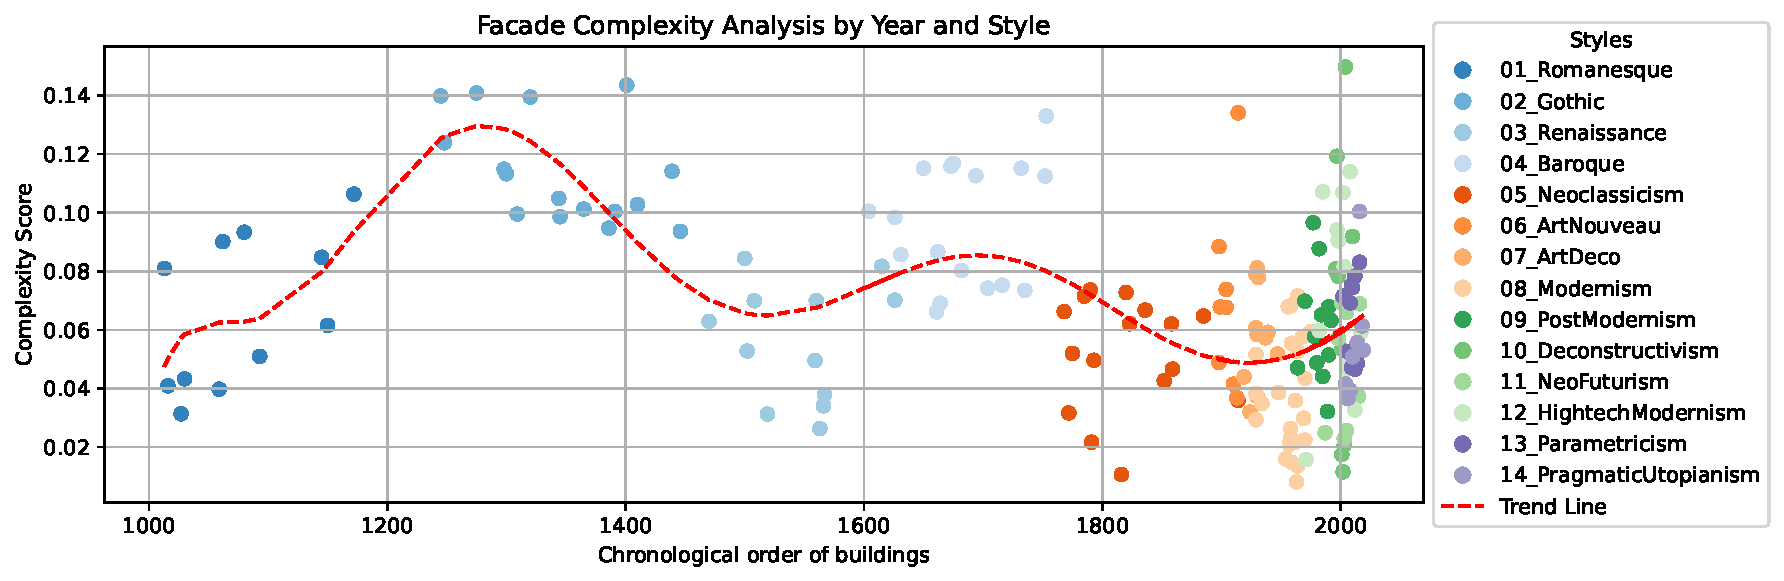
\includegraphics[width= \linewidth]{Graphs/complexitygraph}
          \caption{Contemporary architecture. An era of exploration. (from left to right) Desconstructivism, Neofuturism, High-tech modernism, Parametricism, Pragmatic utopinaism.  (\textit{Images edited from source)}}
          \label{fig:complexitygraph}
        \end{figure*}




We have previously stated the argument that the history of architecture, and the essence of architecture evolution, consists of an ever-changing interplay between simplicity and complexity.

we have explored the theoretical definition and revisioned the different approach towards facades and ornamentation from the perspective of some of the most prominant architectural style across history and the views of their most recognized representatives.

the conclusion from this literature analysis was that the current trend in architecture tilts towards a new revival of complexity however it might look like a suibjective view and insinuate perhaps some biased towards this outcome .

for this reason an additional quantitatvie analysis using Image complexity analysis was conducted using as input images of the most representative buildings across epochs and styles.

For this the complexity image analysis that assigns a complexity value governed by the complexity definition that Complexity of an image is governed by spatial, frequency and color information present in the image.

Scanpath based image complexity analysis determines human visual behavior that could lead to development of interactive and intelligent systems.\cite{Ishrat2020}

The objective of current research work is to establish the complexity of the given set of images while target objects are searched and to present analysis ofgaze search pattern.
To achieve these objectives a remote gaze estimation and analysis model has been proposed for scanpath identification and analysis.\cite{Ishrat2020}

%% Figure of Complexity graph
     \begin{figure*}[htb]
          \centering
          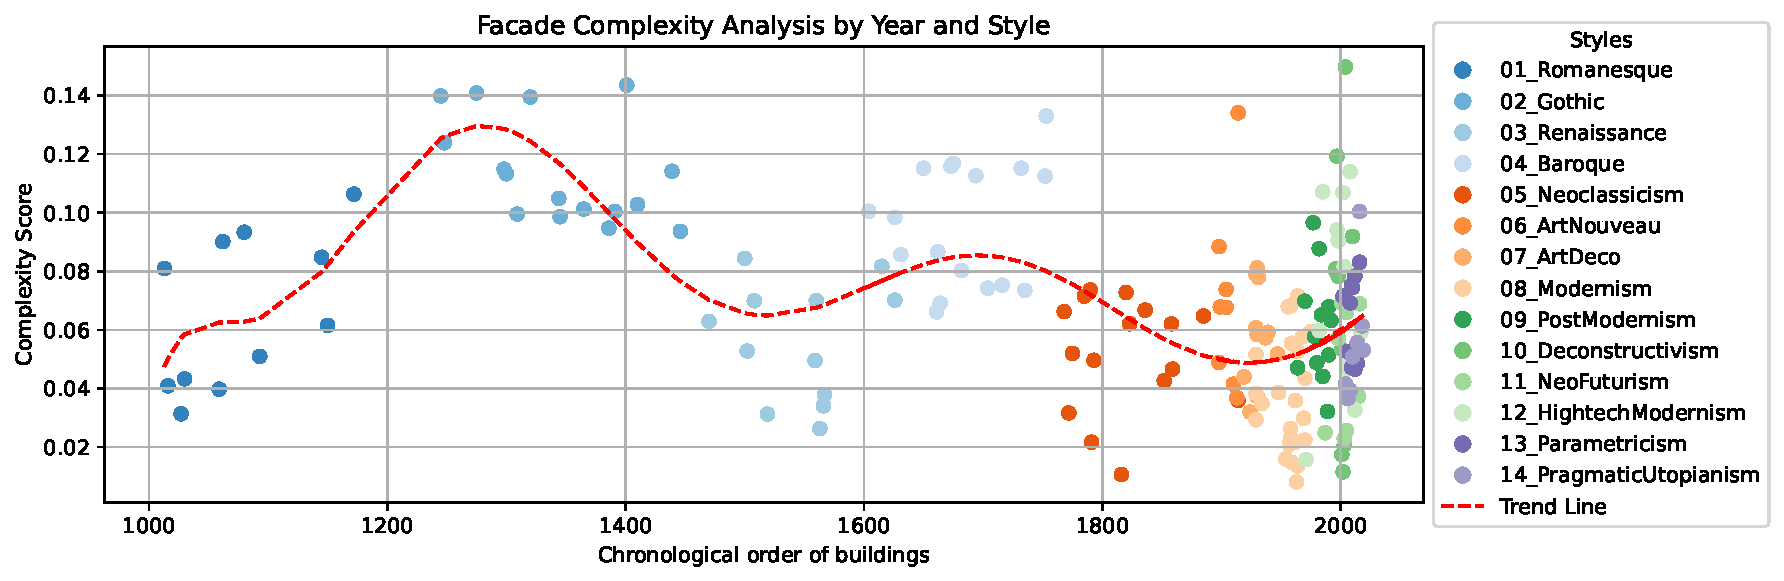
\includegraphics[width= \linewidth]{Graphs/complexitygraph}
          \caption{Contemporary architecture. An era of exploration. (from left to right) Desconstructivism, Neofuturism, High-tech modernism, Parametricism, Pragmatic utopinaism.  (\textit{Images edited from source)}}
          \label{fig:complexitygraph}
        \end{figure*}




We have previously discussed the argument that the architectural evolution, throughout history, has been characterized by a continual interplay between simplicity and complexity.
This notion has been substantiated by our exploration of the theoretical definitions and varied approaches to facades and ornamentation within the context of prominent architectural styles and the perspectives of their eminent architects.

Our literature review has consistently pointed towards a prevailing trend in contemporary architecture, suggesting a resurgence of complexity in architectural design.
However, to ensure our findings are not purely subjective or biased towards this conclusion, we have conducted a quantitative analysis using Image Complexity Analysis.
This rigorous analysis method utilizes input images of the most iconic and representative buildings from various epochs and styles.

Through Image Complexity Analysis, we assign a quantitative complexity value to these architectural images.
This complexity value is derived from a comprehensive examination of spatial intricacies, frequency patterns, and color information present within, based on the research strategy by Ishra et al\cite{Ishrat2020}.

By employing this quantitative approach, we aim to provide an objective measure of the shift from simplicity towards complexity in architecture, further strengthening the thesis of an impending era characterized by architectural intricacy and richness in facades and ornamentation.

The results are visually depicted in Figure\ref{fig:complexitygraph}, where a discernible upward trendline emerges, particularly noticeable since the late 20th century.
This graphical representation unmistakably illustrates a growing inclination towards architecturally complex designs, further corroborating the conclusion drawn from our extensive literature review.

%% Figure of Complexity graph
     \begin{figure*}[htb]
          \centering
          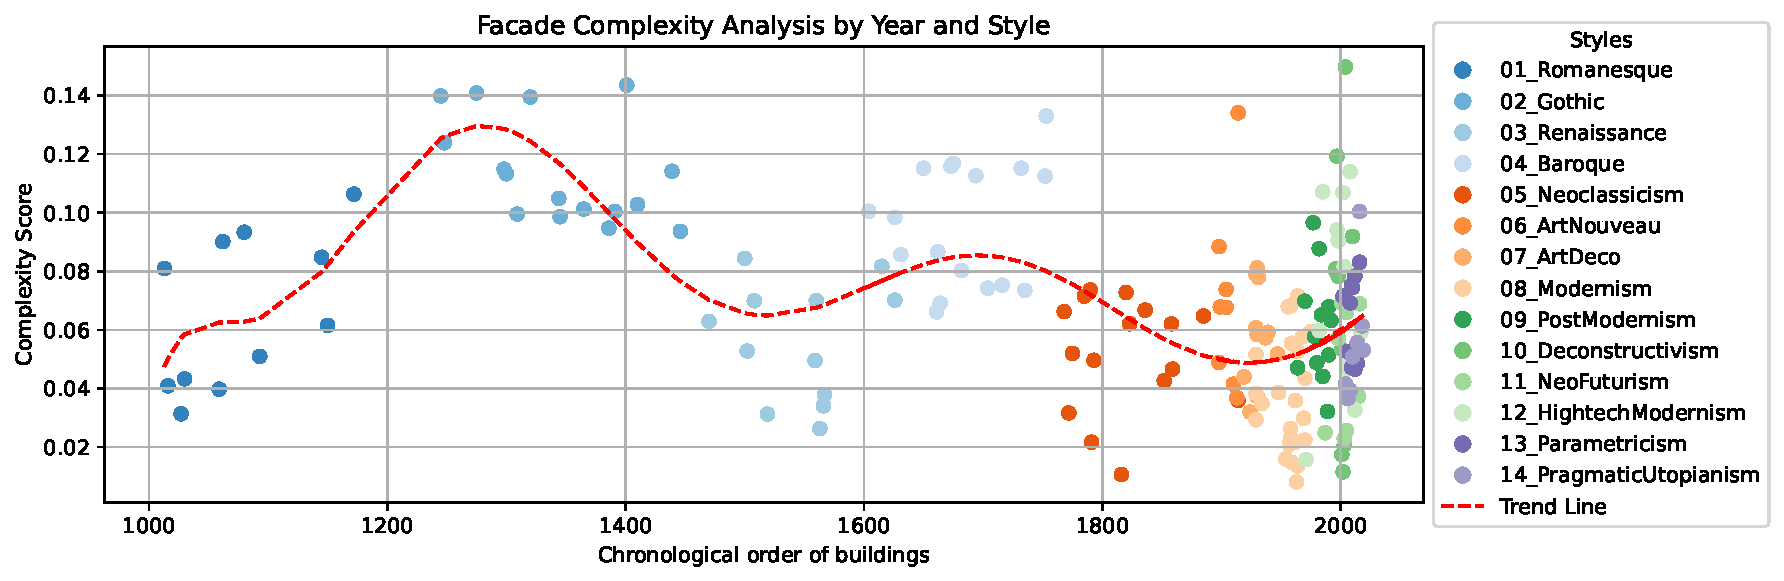
\includegraphics[width= \linewidth]{Graphs/complexitygraph}
          \caption{Contemporary architecture. An era of exploration. (from left to right) Desconstructivism, Neofuturism, High-tech modernism, Parametricism, Pragmatic utopinaism.  (\textit{Images edited from source)}}
          \label{fig:complexitygraph}
        \end{figure*}


=========

 Complexity of an image is governed by spatial, frequency and color information present in the image.\cite{Ishrat2020}

Scanpath based image complexity analysis determines human visual behavior that could lead to development of interactive and intelligent systems.\cite{Ishrat2020}

The objective of current research work is to establish the complexity of the given set of images while target objects are searched and to present analysis ofgaze search pattern.
To achieve these objectives a remote gaze estimation and analysis model has been proposed for scanpath identification and analysis.\cite{Ishrat2020}




